\documentclass[tikz]{standalone}
\usepackage{pgfplots}
\begin{document}
	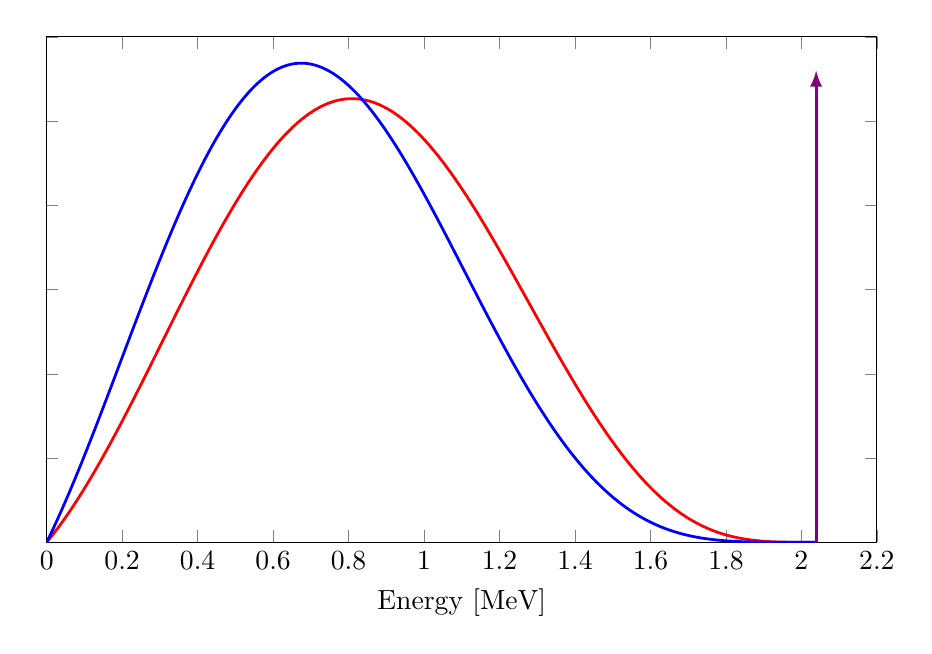
\begin{tikzpicture}
		\begin{axis}[
					%mlineplot,
					width=\textwidth, height=8cm,
					xmin=0, xmax=2.2,
					ymin=0, ymax=0.6,
					samples=200,
					xlabel=Energy {[}MeV{]},
					yticklabels={,,},
					%ylabel=a.u.
					]
			\addplot [mark=none, color=red, line width=1pt, domain=0:2.039]
				{x/0.511*(4-x/0.511)^4*((x/0.511)^4+10*(x/0.511)^3+40*(x/0.511)^2+60*(x/0.511)+30)/27814};
			\addplot [mark=none, color=blue, line width=1pt, domain=0:2.039]
				{x/0.511*(4-x/0.511)^5*((x/0.511)^4+10*(x/0.511)^3+40*(x/0.511)^2+60*(x/0.511)+30)/65749};
			\draw[-latex,color=violet, line width=1pt] (axis cs:2.039,0) -- (axis cs:2.039,0.56);
		\end{axis}
	\end{tikzpicture}
\end{document}
